\documentclass[11pt]{article}
\usepackage[a4paper,margin=26mm]{geometry}
\usepackage[T1]{fontenc}
\usepackage{lmodern,microtype,amsmath,amssymb,amsthm,mathtools}
\usepackage{booktabs,array,xcolor,tikz,listings}
\usepackage[colorlinks=true,linkcolor=blue!45!black,citecolor=blue!45!black,urlcolor=blue!45!black]{hyperref}
\hypersetup{pdftitle={UT-free monotone polytopes without the star Ewald property},pdfauthor={Research draft prepared for Keio}}
\definecolor{ink}{HTML}{17334A}
\definecolor{pale}{HTML}{EAF1F6}
\newtheorem{theorem}{Theorem}[section]
\newtheorem{lemma}[theorem]{Lemma}
\newtheorem{corollary}[theorem]{Corollary}
\theoremstyle{remark}\newtheorem{remark}[theorem]{Remark}
\newcommand{\Z}{\mathbb Z}
\newcommand{\R}{\mathbb R}
\newcommand{\E}{\mathcal E}
\newcommand{\Star}{\operatorname{Star}}
\newcommand{\st}{\operatorname{star}}
\newcommand{\one}{\mathbf1}
\DeclareMathOperator{\Verts}{Vert}
\lstset{basicstyle=\ttfamily\scriptsize,breaklines=true,columns=fullflexible,
keepspaces=true,showstringspaces=false,frame=single,rulecolor=\color{black!20},
backgroundcolor=\color{black!2},aboveskip=10pt,belowskip=10pt}
\title{\textbf{UT-free monotone polytopes\\without the star Ewald property}\\[5pt]
\large An explicit family with arbitrarily long lattice edges}
\author{Research draft prepared for Keio}
\date{7 November 2026}
\begin{document}
\maketitle
\begin{abstract}
For every integer \(r\ge2\), we construct a smooth reflexive polytope \(P_r\)
of dimension \(5r+1\) with \(5r+4\) facets. Every vertex belongs to
\(-\one+r\Z^{5r+1}\), so every edge has lattice length divisible by \(r\).
In particular \(P_r\) has no unimodular triangular two-face. Nevertheless,
an explicit face of dimension \(2r-2\) fails the star Ewald condition:
the active facet heights force a prospective symmetric lattice point
to have one coordinate equal to \(-2\) or \(3\).
We also prove that \(P_r\) satisfies the strong Ewald condition and that
its polar has full vertex minors of absolute values \(2\) and \(3\).
The eleven-dimensional member therefore refutes the star Ewald assertion
in Tu's Conjecture~2, and products give examples in every dimension at
least eleven. The six-dimensional seed and the wedge operation have
known antecedents in Paffenholz--McDuff and Haase--Melnikov.
The additional result is an explicit extension retaining the obstruction
while forcing arbitrary lattice edge divisibility. Historical priority
for that extension is not certified here.
\end{abstract}

\section{The exact target and the construction}

A \emph{monotone polytope} is a smooth reflexive lattice polytope, with
smoothness understood in the Delzant sense: the primitive edge directions
at each vertex form a lattice basis. A polytope is \emph{UT-free} when
none of its two-dimensional faces is a unimodular triangle.
Tu's Conjecture~2 in \cite{Tu24}, repeated in \cite{Tu25}, asserts that
UT-free monotone polytopes are duals of unimodular smooth Fano polytopes,
and in particular satisfy the three Ewald conditions.
We address the star assertion in its original form:
\begin{equation}\label{eq:target}
 P\text{ monotone and UT-free}\quad\Longrightarrow\quad
 P\text{ is star Ewald}.
\end{equation}
The 2024 text has an apparent extra word in the phrase describing
the three conditions; the 2025 report states the three Ewald conditions
without that ambiguity. Both sources explicitly define the star condition.

Fix an integer \(r\ge1\), and put
\[
 p=r+1,\qquad q=2r,\qquad \ell=2r-1,\qquad D=5r+1.
\]
Use coordinates
\[
 a\in\R^p,\quad b\in\R^q,\quad t\in\R^\ell,\quad s\in\R,
 \qquad A=\sum_i a_i,\quad B=\sum_jb_j,\quad T=\sum_\nu t_\nu .
\]
Define
\begin{equation}\label{eq:polytope}
\boxed{\quad
P_r=\left\{(a,b,t,s):
\begin{array}{l}
a_i,b_j,t_\nu,s\ge-1,\\
T\le1,\quad A+s+3T\le1,\quad B+s+2T\le1
\end{array}
\right\}.\quad}
\end{equation}

\begin{theorem}\label{thm:main}
For every integer \(r\ge1\), the following statements hold.
\begin{enumerate}
\item \(P_r\) is \(D\)-dimensional, smooth and reflexive. It has
\(D+3=5r+4\) primitive irredundant facets and \(4r^3+14r^2+7r\) vertices.
\item Every vertex lies in \(-\one+r\Z^D\). Every edge has lattice length
a positive multiple of \(r\).
\item \(P_r\) is strong Ewald but is not star Ewald. An explicit failing face is
\begin{equation}\label{eq:badface}
 F_r=\{a_i=b_j=-1,\ s=4r-1,\ T=1-r\}\cap P_r .
\end{equation}
It is a simplex of dimension \(2r-2\), with edge length \(r\) when \(r\ge2\).
\item The vertex configuration of the polar has full minors of absolute
values \(2\) and \(3\), so it is not unimodular.
\end{enumerate}
Consequently \(P_r\) is UT-free for \(r\ge2\), and \(P_2\) is an
eleven-dimensional counterexample to \eqref{eq:target}.
\end{theorem}

All statements are proved below by explicit formulas valid for every
\(r\); computation is supplementary.
This does not refute Ewald's original 1988 conjecture.
Indeed we exhibit a lattice basis in \(\E(P_r)\) and prove the stronger
facet-by-facet basis property.

\paragraph{Attribution and scope.}
After a coordinate permutation, \(P_1\) is the six-dimensional
Paffenholz example discussed by McDuff
\cite[Section~2.1, Lemma~2.6]{McDuff11}.
Wedges and repeated facet splitting are established constructions
\cite{HM06,McDuff11}. That seed has unimodular triangular faces.
The additional conclusion here is preservation of its star obstruction
together with \(\Verts(P_r)\subset-\one+r\Z^D\).
We do not claim a new wedge operation or the first non-star monotone
polytope. Section~\ref{sec:priority} records the novelty boundary.

\section{A facet-height criterion}

For a monotone polytope
\(P=\{x\in\R^d:\langle n_i,x\rangle\le1,\ 1\le i\le m\}\),
with primitive integral outward normals, its \emph{Ewald set} is
\[
 \E(P)=P\cap(-P)\cap\Z^d
 =\{x\in\Z^d:|\langle n_i,x\rangle|\le1\ \text{for all }i\}.
\]
Weak Ewald means that \(\E(P)\) contains a lattice basis.
Strong Ewald means that \(\E(P)\) on each facet contains a lattice basis.

For a face \(F\), let \(\Star(F)\) be the union of the facets containing
\(F\), let \(\st(F)\) be the union of the ridges containing \(F\), and
put \(\Star^*(F)=\Star(F)\setminus\st(F)\).
The face is star Ewald if some \(\lambda\in\E(P)\) satisfies
\[
       \lambda\in\Star^*(F),\qquad-\lambda\notin\Star(F).
\]
The polytope is star Ewald when every nonempty proper face is.
These are the definitions used in \cite{Tu24,CPS26}.

\begin{lemma}\label{lem:star}
Let \(I(F)\) index the facets containing \(F\).
A point \(\lambda\in\E(P)\) is a star witness for \(F\) if and only if
\[
       \big(\langle n_i,\lambda\rangle\big)_{i\in I(F)}
\]
has exactly one entry equal to \(1\), with all other entries zero.
\end{lemma}
\begin{proof}
The entries are integers in \(\{-1,0,1\}\).
The condition on \(-\lambda\) excludes \(-1\), and membership in
\(\Star(F)\) requires a \(1\).
In a simple polytope, two distinct facets containing \(F\) intersect
in a ridge containing \(F\). Membership in \(\Star^*(F)\) therefore
allows exactly one \(1\). The converse is immediate.
\end{proof}
This criterion will exclude every possible witness, without a height
cutoff or a search through a finite portion of the lattice.

\section{A fixed pentagon describes every vertex}

Set
\[
 a_i=r\alpha_i-1,\quad b_j=r\beta_j-1,\quad
 t_\nu=r\tau_\nu-1,\quad s=r\sigma-1.
\]
This is a vertex description, not a claimed unimodular equivalence.
It gives \(P_r=rR_r-\one\), where
\begin{equation}\label{eq:rescaled}
 R_r=\left\{\begin{array}{l}
 \alpha_i,\beta_j,\tau_\nu,\sigma\ge0,\quad U:=\sum_\nu\tau_\nu\le2,\\
 \sum_i\alpha_i+\sigma+3U\le7,\quad
 \sum_j\beta_j+\sigma+2U\le6
 \end{array}\right\}.
\end{equation}
The projection to \((\sigma,U)\) is the pentagon
\[
 K=\{(\sigma,U):\sigma\ge0,\ 0\le U\le2,\
                 \sigma+3U\le7,\ \sigma+2U\le6\},
\]
whose vertices are
\[
              (0,0),\ (6,0),\ (4,1),\ (1,2),\ (0,2).
\]

\begin{figure}[ht]
\centering
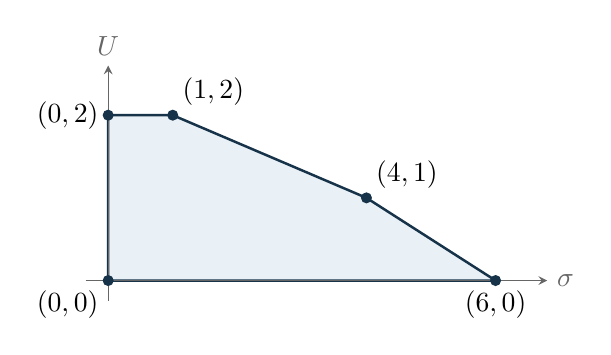
\begin{tikzpicture}[x=0.82cm,y=1.05cm,>=stealth]
 \filldraw[fill=pale,draw=ink,line width=0.9pt]
 (0,0)--(6,0)--(4,1)--(1,2)--(0,2)--cycle;
 \draw[->,black!60] (-.35,0)--(6.8,0) node[right] {\(\sigma\)};
 \draw[->,black!60] (0,-.25)--(0,2.6) node[above] {\(U\)};
 \foreach \x/\y in {0/0,6/0,4/1,1/2,0/2}
  \fill[ink] (\x,\y) circle (2pt);
 \node[below left] at (0,0) {\((0,0)\)};
 \node[below] at (6,0) {\((6,0)\)};
 \node[above right] at (4,1) {\((4,1)\)};
 \node[above right] at (1,2) {\((1,2)\)};
 \node[left] at (0,2) {\((0,2)\)};
\end{tikzpicture}
\caption{The pentagon is fixed. Increasing \(r\) changes the numbers
of coordinates in its simplex fibers.}
\end{figure}

Over \((\sigma,U)\), the fiber is the product of
\begin{align*}
 &\alpha\ge0,\quad \sum_i\alpha_i\le L_a:=7-\sigma-3U,\\
 &\beta\ge0,\quad \sum_j\beta_j\le L_b:=6-\sigma-2U,\\
 &\tau\ge0,\quad \sum_\nu\tau_\nu=U.
\end{align*}

\begin{lemma}\label{lem:vertices}
The vertices of \(R_r\) are exactly the fiber vertices over the five
vertices of \(K\). In particular, every vertex of \(R_r\) is integral.
\end{lemma}
\begin{proof}
Include the slack coordinates \(L_a-\sum\alpha_i\) and
\(L_b-\sum\beta_j\). Barycentric proportions describe each fiber point.
If its base point lies in a nontrivial segment of its minimal face in
\(K\), keep those proportions fixed and vary the base point.
The fiber sizes are affine, so this produces an affine segment through
the given point in \(R_r\).
A zero fiber size causes no exception: a nonnegative affine function
vanishing at a relative interior point of a face vanishes on that face.
Thus a vertex projects to a vertex of \(K\), and it must be a fiber vertex.
Conversely, any convex decomposition of a fiber vertex over a base
vertex stays in that fiber and is trivial.
A fiber vertex allocates its whole size to one coordinate, possibly
the slack coordinate. The base vertices and fiber sizes are integral.
\end{proof}

\begin{table}[ht]
\centering\renewcommand{\arraystretch}{1.15}
\begin{tabular}{@{}cccc l@{}}
\toprule
\((\sigma,U)\)&\(L_a\)&\(L_b\)&\(U\)&Number of vertices\\
\midrule
\((0,0)\)&7&6&0&\((r+2)(2r+1)\)\\
\((6,0)\)&1&0&0&\(r+2\)\\
\((4,1)\)&0&0&1&\(2r-1\)\\
\((1,2)\)&0&1&2&\((2r+1)(2r-1)\)\\
\((0,2)\)&1&2&2&\((r+2)(2r+1)(2r-1)\)\\
\bottomrule
\end{tabular}
\caption{Complete vertex enumeration for every \(r\ge1\).}
\label{tab:vertices}
\end{table}

The sum is \(4r^3+14r^2+7r\).
The same description proves
\begin{equation}\label{eq:coset}
                    \Verts(P_r)\subset-\one+r\Z^D.
\end{equation}

\section{Smoothness, reflexivity, and UT-freeness}

The system \eqref{eq:rescaled} is bounded.
Every inequality in \eqref{eq:polytope} is strict at the origin, giving
full dimension.

\begin{lemma}\label{lem:smooth}
Exactly \(D\) facets meet at each vertex of \(P_r\), and their primitive
outward normals have determinant \(\pm1\).
\end{lemma}
\begin{proof}
Work in \(R_r\), whose facet normals are the same.
First eliminate the zero coordinates with their lower unit normals.
If an \(\alpha\) or \(\beta\) coordinate is positive, it is the only
positive coordinate in its block; its upper inequality supplies
a unit pivot in that coordinate.
When \(U>0\), precisely one \(\tau\) coordinate is positive.

The five cases in Table~\ref{tab:vertices} leave the following residual
matrices, respectively:
\[
 (),\qquad (1),\qquad
 \begin{pmatrix}1&3\\1&2\end{pmatrix},\qquad
 \begin{pmatrix}1&3\\0&1\end{pmatrix},\qquad (1).
\]
The empty determinant is \(1\); all others are \(\pm1\).
In the middle case the remaining coordinates are \(\sigma\) and the
positive \(\tau\) coordinate, and the two upper inequalities supply
the displayed matrix.
At \((1,2)\), the first upper inequality and \(U=2\) remain after
any \(\beta\) carrier is eliminated.
The other cases have only triangular unit pivots.
The list accounts for every active inequality and has exactly \(D\)
independent rows in each case.
\end{proof}

Every lower-coordinate inequality is a facet: set that coordinate to
\(-1\) and all others to zero.
For the \(A\) upper facet, use \(a_1=1\) and all other coordinates zero;
the analogous point works for the \(B\) upper facet.
For \(T=1\), take all \(t_\nu=1/\ell\) and all \(a_i,b_j,s\) slightly
greater than \(-1\), making both other upper inequalities strict.
All \(D+3\) inequalities are therefore irredundant; their normals
are primitive.

The vertices are integral by Lemma~\ref{lem:vertices}.
All primitive facet equations of \(P_r\) have constant \(1\), and the
origin is interior. The polar is thus a convex hull of integral
normals and is integral, proving reflexivity.
Lemma~\ref{lem:smooth} proves smoothness and hence monotonicity.

For distinct edge endpoints \(v,w\), the lattice length is the greatest
common divisor of the coordinates of \(v-w\), with signs and zero
entries ignored. Equation~\eqref{eq:coset} makes it a positive multiple
of \(r\). For \(r\ge2\), every edge contains an interior lattice point.
A unimodular triangle has primitive edges, so \(P_r\) is UT-free.

\section{The star obstruction and polar determinants}

The face \(F_r\) is obtained by setting every \(a_i,b_j=-1\) and
making the two upper inequalities involving \(A,B\) equalities.
Solving gives \(s=4r-1,\ T=1-r\).
The remaining coordinates satisfy
\[
 t_\nu+1\ge0,\qquad\sum_{\nu=1}^{2r-1}(t_\nu+1)=r.
\]
Thus \(F_r\) is a \((2r-2)\)-simplex, of edge length \(r\) for \(r\ge2\).
At its relative interior \(t_\nu>-1\), \(s>-1\), and \(T<1\).
Its containing facets are exactly the \(a,b\) lower facets and the
two upper facets involving \(A,B\).

If \(\lambda\in\E(P_r)\) were a star witness, Lemma~\ref{lem:star}
would make all their heights zero except for one height \(1\).
Group the \(a\) lower facets with the \(A\) upper facet, and the \(b\)
lower facets with the \(B\) upper facet.
The two sums of heights, \(\varepsilon,\delta\), obey
\[
       (\varepsilon,\delta)\in\{(1,0),(0,1)\}.
\]
Cancellation in the groups gives
\[
 s(\lambda)+3T(\lambda)=\varepsilon,\qquad
 s(\lambda)+2T(\lambda)=\delta.
\]
Consequently
\begin{equation}\label{eq:contradiction}
               s(\lambda)=3\delta-2\varepsilon\in\{-2,3\}.
\end{equation}
But both \(\lambda,-\lambda\) satisfy \(s\ge-1\), so
\(|s(\lambda)|\le1\), a contradiction. This proves the star failure
for every \(r\).

For the polar, use \(P_r^\circ=\{y:\langle y,x\rangle\le1
\text{ for all }x\in P_r\}\).
Its vertices are the primitive facet normals.
In the negative coordinate matrix \(-I_D\), replace one \(t_\nu\) row
by the normal of \(A+s+3T\le1\). The determinant has absolute value \(3\).
Replacing it by the normal of \(B+s+2T\le1\) gives absolute value \(2\).
A unimodular coordinate change preserves these absolute determinants.
The selected full subsets are not facets of the polar; smoothness
requires unit determinants for actual facets, whereas the USFP
definition requires them for every full subset.

Tu's negative-polar convention gives \(-P_r^\circ\).
The map \(-I\) is unimodular, so the convention has no effect here.

\section{Strong Ewald is preserved}

A direct weak Ewald basis is
\begin{equation}\label{eq:weakbasis}
 \{e_{a_i}\}_i\cup\{e_{b_j}\}_j\cup\{e_s\}\cup
 \{e_{t_\nu}-e_{a_1}-e_s\}_\nu .
\end{equation}
Elementary column operations give determinant \(1\).
Every vector has all facet heights in \(\{-1,0,1\}\).
For the last type, the three upper heights are \(1,1,1\).
Thus the construction explicitly satisfies Ewald's original condition.

\begin{lemma}[Strong Ewald under facet splitting]\label{lem:splitstrong}
Let \(Q=\{x:n_i x\le1\}\) be monotone and strong Ewald, with the
\(n_i x\le1\) its primitive irredundant facet inequalities.
Replace each inequality by
\[
 z_{i,j}\ge-1\ (1\le j<k_i),\qquad
 n_i x+\sum_{j<k_i}z_{i,j}\le1,
\]
where the \(k_i\) are positive integers.
If the resulting polytope \(L\) is monotone and these are its facets,
then it is strong Ewald.
\end{lemma}
\begin{proof}
Fix a top facet in block \(i\), and choose a lattice basis
\(x_1,\ldots,x_d\) in \(\E(Q)\cap\{n_i x=1\}\).
Embed these vectors with new coordinates zero.
For every new coordinate in block \(i\), add its unit vector.
For a new coordinate in a different block \(g\), add
\((x_1,\eta e_{g,j})\), where \(\eta=\pm1\) is chosen so that
\(n_gx_1+\eta\in[-1,1]\). Such a choice exists because
\(n_gx_1\in\{-1,0,1\}\).
All these vectors are Ewald points on the chosen top facet.
Subtracting the first embedded vector when appropriate leaves a
block triangular basis of determinant \(\pm1\).

The integral linear involution
\(z_{i,j}\mapsto -n_i x-\sum_hz_{i,h}\), with other coordinates fixed,
preserves \(L\), has determinant \(-1\), and exchanges the top facet
with the corresponding lower facet. It transfers the basis to every
lower facet.
\end{proof}

\begin{lemma}\label{lem:seedstrong}
The six-dimensional member \(P_1\) is strong Ewald.
\end{lemma}
\begin{proof}
Use seed coordinates
\((a_1,a_2,b_1,b_2,s,t_1)=(x_1,x_2,x_3,x_4,x_5,x_6)\).
The upper normals are
\[
 e_6,\qquad c=(1,1,0,0,1,3),\qquad d=(0,0,1,1,1,2).
\]
Put \(w=e_6-e_1-e_5\).
For \(x_i=-1\), \(1\le i\le5\), use the six vectors
\[
 -e_i,\quad\{-e_i+e_j:1\le j\le5,\ j\ne i\},\quad u_i,
\]
where \(u_i=w\) for \(i=1,5\), and \(u_i=w-e_i\) otherwise.
Every normal height is in \(\{-1,0,1\}\).
The first five vectors form a basis in the first five coordinates,
and the last has sixth coordinate \(1\), so the determinant is \(\pm1\).
For \(x_6=1\), use \(v,v+e_1,\ldots,v+e_5\), where
\(v=(-1,-1,-1,-1,-1,1)\).
These are Ewald points of determinant \(\pm1\).
Their negatives handle \(x_6=-1\).
Finally the separate involutions
\[
 x_1\mapsto-x_1-x_2-x_5-3x_6,\qquad
 x_3\mapsto-x_3-x_4-x_5-2x_6
\]
with other coordinates fixed preserve \(P_1\), have determinant \(-1\),
and exchange the corresponding lower and upper facets.
This treats all nine facets.
\end{proof}

Split the lower seed facets for \(x_2,x_3,x_4,x_6\) into blocks of
sizes \(r,r,r,2r-1\).
For a split lower facet \(-x_i\le1\), the coordinates
\[
 z_{i,1},\ldots,z_{i,k_i-1},\quad x_i-\sum_jz_{i,j}
\]
all have lower bound \(-1\), sum to \(x_i\), and are obtained by a
unimodular transformation.
Regrouping them makes the old coordinates
\[
 x_1=a_1,\quad x_2=\sum_{i=2}^{r+1}a_i,\quad
 x_3=\sum_{j=1}^r b_j,\quad x_4=\sum_{j=r+1}^{2r}b_j,\quad
 x_5=s,\quad x_6=T.
\]
The resulting inequalities are exactly \eqref{eq:polytope}.
Monotonicity was independently proved above.
Lemmas~\ref{lem:splitstrong} and \ref{lem:seedstrong} now prove strong
Ewald for every \(P_r\), completing Theorem~\ref{thm:main}.

\section{Consequences, exact checks, and prior results}

\begin{corollary}
For every dimension \(N\ge11\) there is a UT-free monotone polytope
that is strong Ewald and not star Ewald.
No dimension-independent lower bound on lattice edge length forces a
monotone polytope to be star Ewald.
\end{corollary}
\begin{proof}
Use \(P_2\times[-1,1]^{N-11}\).
Products preserve smoothness and reflexivity, and every edge has
length at least \(2\). A star witness for
\(F_2\times[-1,1]^{N-11}\) would project to one for \(F_2\).

Strong Ewald is preserved under products: for a facet \(H\times Q\),
embed an Ewald basis on \(H\), and append one fixed member of that
basis paired with each member of an Ewald basis of \(Q\).
The resulting basis is contained in that facet. The other facet type
is symmetric. The final assertion follows by taking \(r\) arbitrarily
large in Theorem~\ref{thm:main}.
\end{proof}

We do not claim that eleven is the minimum possible dimension.
The last assertion concerns dimension-independent bounds only.

\subsection{Exact verification}
For \(r=2\), all \(\binom{14}{11}=364\) candidate normal bases were tested
with exact rational arithmetic. The resulting list agrees with the
analytic description. Separate implementations, including one in
split coordinates, gave the same result.
\begin{center}
\begin{tabular}{@{}lr@{}}
\toprule
Quantity&Exact value\\
\midrule
Dimension&11\\
Primitive irredundant facets&14\\
Vertices&102\\
Edges&561\\
Edges of lengths \(2,4,12,14\)&\(216,\ 255,\ 60,\ 30\)\\
Vertices of the bad face&3\\
Absolute active vertex determinants&1\\
Exhibited polar minors&2 and 3\\
\bottomrule
\end{tabular}
\end{center}
These checks supplement the all-\(r\) proof.
Appendix~\ref{app:code} supplies a compact standard-library verifier.
The manuscript is not a proof-assistant formalization and has not
received external peer review.

\subsection{The novelty boundary}\label{sec:priority}
The known seed is not UT-free: its face
\(x_3=x_4=x_5=-1,\ x_6=1\) is the unit triangle with free-coordinate
vertices \((-1,-1),(0,-1),(-1,0)\).
Products retain such a face.
The present construction changes the dimension and facet
multiplicities while retaining monotone normalization, and forces
all vertices into one residue class modulo \(r\).

A separate, simpler overlap affects the dual-USFP inclusion alone.
The known simplex--segment bundle
\[
 |x|\le1,\quad y_i\ge-1\ (1\le i\le3),\quad
             2x+y_1+y_2+y_3\le1
\]
is UT-free by \cite[Proposition~5.14]{CPS26}.
Its polar has a determinant-two minor, as in the family of
\cite[Example~7.1]{Tu26}. These facts already imply a counterexample
to the inclusion, but do not give a non-star example:
the SSB family satisfies star Ewald \cite[Proposition~5.16]{CPS26}.
The additional claim examined here is specifically the UT-free,
non-star family with arbitrary edge divisibility.

The primary-source audit inspected the conjecture, its 2025 repetition,
the wedge antecedents, CPS, and the three available six-dimensional
examples on Paffenholz's page \cite{PaffenholzData}.
Each of those three has a unimodular triangular face.
The linked seven-dimensional archive was not retrievable.
Equivalent descriptions involving long edges, Fano index, and probe
failure were also considered. No inspected source supplied the combined
all-\(r\) conclusion. This is a bounded search, not proof of priority.

\begin{center}\small
\begin{tabular}{@{}p{.09\linewidth}p{.84\linewidth}@{}}
\toprule
Criterion&Established scope\\
\midrule
G1&The star assertion occurs in Tu's prior Conjecture~2.\\
G2&The original UT-free, monotone, and star definitions are unchanged.\\
G3&The cited sources propose the conjecture; historical absence of an
earlier resolution is not certified.\\
G4&The counterexample and the full \(r\)-family have unconditional
analytic proofs.\\
G5&Vertex congruence and a surviving height obstruction yield an actual
new-result candidate using known wedges. A historically new fundamental
method is not claimed.\\
G6&Known overlapping constructions are attributed. First-discovery
status remains unverified.\\
\bottomrule
\end{tabular}
\end{center}

\appendix
\section{A compact exact verifier}\label{app:code}
The following Python~3 code needs no third-party packages.
It verifies the \(r=2\) vertices, simplicity, smoothness, parity,
edge lengths, bad face, Ewald basis, and nonunit polar minors.
The analytic proof additionally establishes facet irredundancy
and every statement for all \(r\).

\begin{lstlisting}[language=Python]
from fractions import Fraction as F
from itertools import combinations
from collections import Counter
from math import gcd
from functools import reduce

r = 2
p, q, h = r+1, 2*r, 2*r-1
D = p+q+h+1
ia = list(range(p))
ib = list(range(p, p+q))
it = list(range(p+q, p+q+h))
S = D-1

def unit(j):
    v = [0]*D
    v[j] = 1
    return v

def dot(a, b):
    return sum(x*y for x, y in zip(a, b))

def solve(M, rhs):
    n = len(M)
    B = [[F(x) for x in row] + [F(rhs[i])]
         for i, row in enumerate(M)]
    det = F(1)
    for j in range(n):
        k = next((k for k in range(j, n) if B[k][j]), None)
        if k is None:
            return None, F(0)
        if k != j:
            B[k], B[j] = B[j], B[k]
            det = -det
        z = B[j][j]
        det *= z
        B[j] = [x/z for x in B[j]]
        for k in range(n):
            if k != j:
                z = B[k][j]
                B[k] = [x-z*y for x, y in zip(B[k], B[j])]
    return tuple(B[i][-1] for i in range(n)), det

N = [[-x for x in unit(j)] for j in range(D)]
nt = [int(j in it) for j in range(D)]
na = [int(j in ia)+int(j == S)+3*int(j in it)
      for j in range(D)]
nb = [int(j in ib)+int(j == S)+2*int(j in it)
      for j in range(D)]
N += [nt, na, nb]

vertices = {}
for J in combinations(range(D+3), D):
    v, det = solve([N[j] for j in J], [1]*D)
    if v is None or any(dot(n, v) > 1 for n in N):
        continue
    assert all(x.denominator == 1 for x in v)
    active = tuple(i for i, n in enumerate(N) if dot(n, v) == 1)
    assert len(active) == D and abs(det) == 1
    vertices[tuple(map(int, v))] = frozenset(active)

assert len(vertices) == 102
assert all(all((x+1) % r == 0 for x in v) for v in vertices)
assert set().union(*vertices.values()) == set(range(D+3))

edges = Counter()
for v, w in combinations(vertices, 2):
    if len(vertices[v] & vertices[w]) == D-1:
        length = reduce(gcd, (abs(x-y) for x, y in zip(v, w)))
        edges[length] += 1
assert edges == Counter({2:216, 4:255, 12:60, 14:30})

bad = [v for v in vertices
       if all(v[j] == -1 for j in ia+ib)
       and v[S] == 4*r-1 and sum(v[j] for j in it) == 1-r]
assert len(bad) == 3
active_bad = frozenset(ia+ib+[D+1,D+2])
assert frozenset.intersection(*(vertices[v] for v in bad)) == active_bad

ga = [sum(N[i][j] for i in ia+[D+1]) for j in range(D)]
gb = [sum(N[i][j] for i in ib+[D+2]) for j in range(D)]
assert ga == [int(j == S)+3*int(j in it) for j in range(D)]
assert gb == [int(j == S)+2*int(j in it) for j in range(D)]

basis = [unit(j) for j in ia+ib+[S]]
for j in it:
    w = unit(j)
    w[ia[0]] = -1
    w[S] = -1
    basis.append(w)
_, det = solve(list(map(list, zip(*basis))), [0]*D)
assert abs(det) == 1
assert all(abs(dot(n, w)) <= 1 for n in N for w in basis)

for upper, expected in [(na,3), (nb,2)]:
    M = [row[:] for row in N[:D]]
    M[it[0]] = upper
    _, det = solve(M, [0]*D)
    assert abs(det) == expected

print("ALL EXACT CHECKS PASSED")
print("vertices =", len(vertices), "edges =", sum(edges.values()))
print("edge length histogram =", dict(sorted(edges.items())))
\end{lstlisting}

\begin{thebibliography}{9}
\bibitem{Tu24}
B.~Tu, \emph{Unimodular Smooth Fano Polytopes and their Relation with
Ewald Conditions}, arXiv:2409.14678v2, 29 September 2024.
\url{https://arxiv.org/abs/2409.14678}.
\bibitem{Tu25}
B.~Tu, \emph{Unimodular smooth Fano polytopes and their relation with
Ewald conditions}, 21st Mathematics Conference for Young Researchers,
technical report, 2025.
\url{https://www.math.sci.hokudai.ac.jp/~wakate/mcyr/2025/pdf/Tu\%20Binnan.pdf}.
\bibitem{HM06}
C.~Haase and I.~V.~Melnikov,
\emph{The reflexive dimension of a lattice polytope},
Annals of Combinatorics \textbf{10} (2006), 211--217.
\href{https://doi.org/10.1007/s00026-006-0283-9}{doi:10.1007/s00026-006-0283-9}.
\bibitem{McDuff11}
D.~McDuff, \emph{The topology of toric symplectic manifolds},
Geometry \& Topology \textbf{15} (2011), 145--190.
\href{https://doi.org/10.2140/gt.2011.15.145}{doi:10.2140/gt.2011.15.145}.
\bibitem{CPS26}
L.~Crespo, \'{A}.~Pelayo, and F.~Santos,
\emph{Ewald's Conjecture and integer points in algebraic and symplectic
toric geometry},
Proceedings of the London Mathematical Society \textbf{132}(4) (2026), e70144.
\href{https://doi.org/10.1112/plms.70144}{doi:10.1112/plms.70144}.
Preprint arXiv:2310.10366v3 (2024).
\bibitem{Tu26}
B.~Tu, \emph{Unimodular defect and antipodal lattice points of smooth
reflexive polytopes}, arXiv:2610.26125v1, 19 October 2026.
\url{https://arxiv.org/abs/2610.26125}.
\bibitem{PaffenholzData}
A.~Paffenholz, \emph{Examples and Counterexamples to some Conjectures},
primary data page, Star Ewald section.
\url{https://polymake.org/polytopes/paffenholz/www/other.html}.
Accessed 7 November 2026.
\end{thebibliography}
\end{document}

